% Digital Logic Report Template
% Created: 2020-01-10, John Miller

%==========================================================
%=========== Document Setup  ==============================

% Formatting defined by class file
\documentclass[11pt]{article}

% ---- Document formatting ----
\usepackage[margin=1in]{geometry}	% Narrower margins
\usepackage{booktabs}				% Nice formatting of tables
\usepackage{graphicx}				% Ability to include graphics

%\setlength\parindent{0pt}	% Do not indent first line of paragraphs 
\usepackage[parfill]{parskip}		% Line space b/w paragraphs
%	parfill option prevents last line of pgrph from being fully justified

% Parskip package adds too much space around titles, fix with this
\RequirePackage{titlesec}
\titlespacing\section{0pt}{8pt plus 4pt minus 2pt}{3pt plus 2pt minus 2pt}
\titlespacing\subsection{0pt}{4pt plus 4pt minus 2pt}{-2pt plus 2pt minus 2pt}
\titlespacing\subsubsection{0pt}{2pt plus 4pt minus 2pt}{-6pt plus 2pt minus 2pt}

% ---- Hyperlinks ----
\usepackage[colorlinks=true,urlcolor=blue]{hyperref}	% For URL's. Automatically links internal references.

% ---- Code listings ----
\usepackage{listings} 					% Nice code layout and inclusion
\usepackage[usenames,dvipsnames]{xcolor}	% Colors (needs to be defined before using colors)

% Define custom colors for listings
\definecolor{listinggray}{gray}{0.98}		% Listings background color
\definecolor{rulegray}{gray}{0.7}			% Listings rule/frame color

% Style for Verilog
\lstdefinestyle{Verilog}{
	language=Verilog,					% Verilog
	backgroundcolor=\color{listinggray},	% light gray background
	rulecolor=\color{blue}, 			% blue frame lines
	frame=tb,							% lines above & below
	linewidth=\columnwidth, 			% set line width
	basicstyle=\small\ttfamily,	% basic font style that is used for the code	
	breaklines=true, 					% allow breaking across columns/pages
	tabsize=3,							% set tab size
	commentstyle=\color{gray},	% comments in italic 
	stringstyle=\upshape,				% strings are printed in normal font
	showspaces=false,					% don't underscore spaces
}

% How to use: \Verilog[listing_options]{file}
\newcommand{\Verilog}[2][]{%
	\lstinputlisting[style=Verilog,#1]{#2}
}




%======================================================
%=========== Body  ====================================
\begin{document}

\title{ELC 2137 Lab 01: Git and LaTeX Intro}
\author{Yiting Wang}

\maketitle


\section*{Summary}

	In this lab, it talk about two tools that are es-pecially suited for programming.  Git is a version con-trol software that helps you keep track of modifica-tions you make to a code project and collaboratewith others on that project.  LaTeX is a typesettinglanguage that can produce professional-looking doc-uments and makes including code very easy.



\section*{Q\&A}

	\begin{enumerate}
		\item What is your GitHub user name?
		
			yiting-wang1
		
		\item What LaTeX environment produces a bulleted(non-numbered) list?
		
			The bulleted lists are produced by the itemize environment. Each entry must be preceded by the control sequence \verb|\item|.
		
		\item Write the equation \verb| y(t) = 1/2 e^t| using Latex equation formatting.
		
			  \[ y(t) = 1/2 e^t \] 
		
		\item What is the shortcut key for compiling your Latex document?
		
		\begin{itemize}
			\item F5 -- compile to PDF
			\item Starting typing a command, then use arrows to choose the desired auto-complete command, and press Enter.  For example, type \verb|\V| and the first item in the pop-up list should be the \verb|\Verilog| command.
			\item In tables, TeXstudio will highlight things in red when the number of columns specified doesn't match the number of columns you have in a particular row.  Summary: When nothing is red, you have the right number everywhere!
			\item Text formatting, similar to MS Word:
			\begin{itemize}
				\item Ctrl+b = \textbf{bold}
				\item Ctrl+i = \textit{italic}
				\item Ctrl+Shift+t = \texttt{typewritter (monospaced)}
			\end{itemize}
			\item Ctrl+Shift+i = insert ``\verb|\item |''
			\item Standard Windows shortcuts:
			\begin{itemize}
				\item Ctrl+z = undo
				\item Ctrl+y = redo
				\item Ctrl+c = copy
				\item Ctrl+x = cut
				\item Ctrl+v = paste
			\end{itemize}
		\end{itemize}

	\end{enumerate}
	
	
	
\section*{Results}

	Figure 1 is the replication of the table and figure shown in Figure 1.1 in Lab 1 Git and LaTex Intro. It  uses a single figure environment to ensure that the table andimage do not get separated.\\ 
	\begin{figure}[ht]\centering
		\begin{tabular}{c|c|c}
			\toprule
			Binary & Hex & Decimal \\
			\midrule
			0000 & 0 & 0 \\
			0010 & 2 & 2 \\
			0100 & 4 & 4 \\
			0110 & 6 & 6 \\
			1000 & 8 & 8 \\
			1010 & A & 10 \\
			\bottomrule
		\end{tabular}\medskip
		
		\centering
		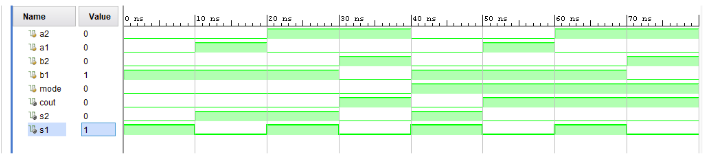
\includegraphics[width=1.0\linewidth]{Lab1F1}
		\caption{Table and simulation waveform to reproduce}
		\label{fig:lab1table}
	\end{figure}
	
	This part is using the trim and cropoptions for the \verb|\includegraphics| command to just get the part of the image people want. Figure 2 is the original one, and Figure 3 is the logo cropping the top and bottom.\\
	\begin{figure}[ht]\centering
		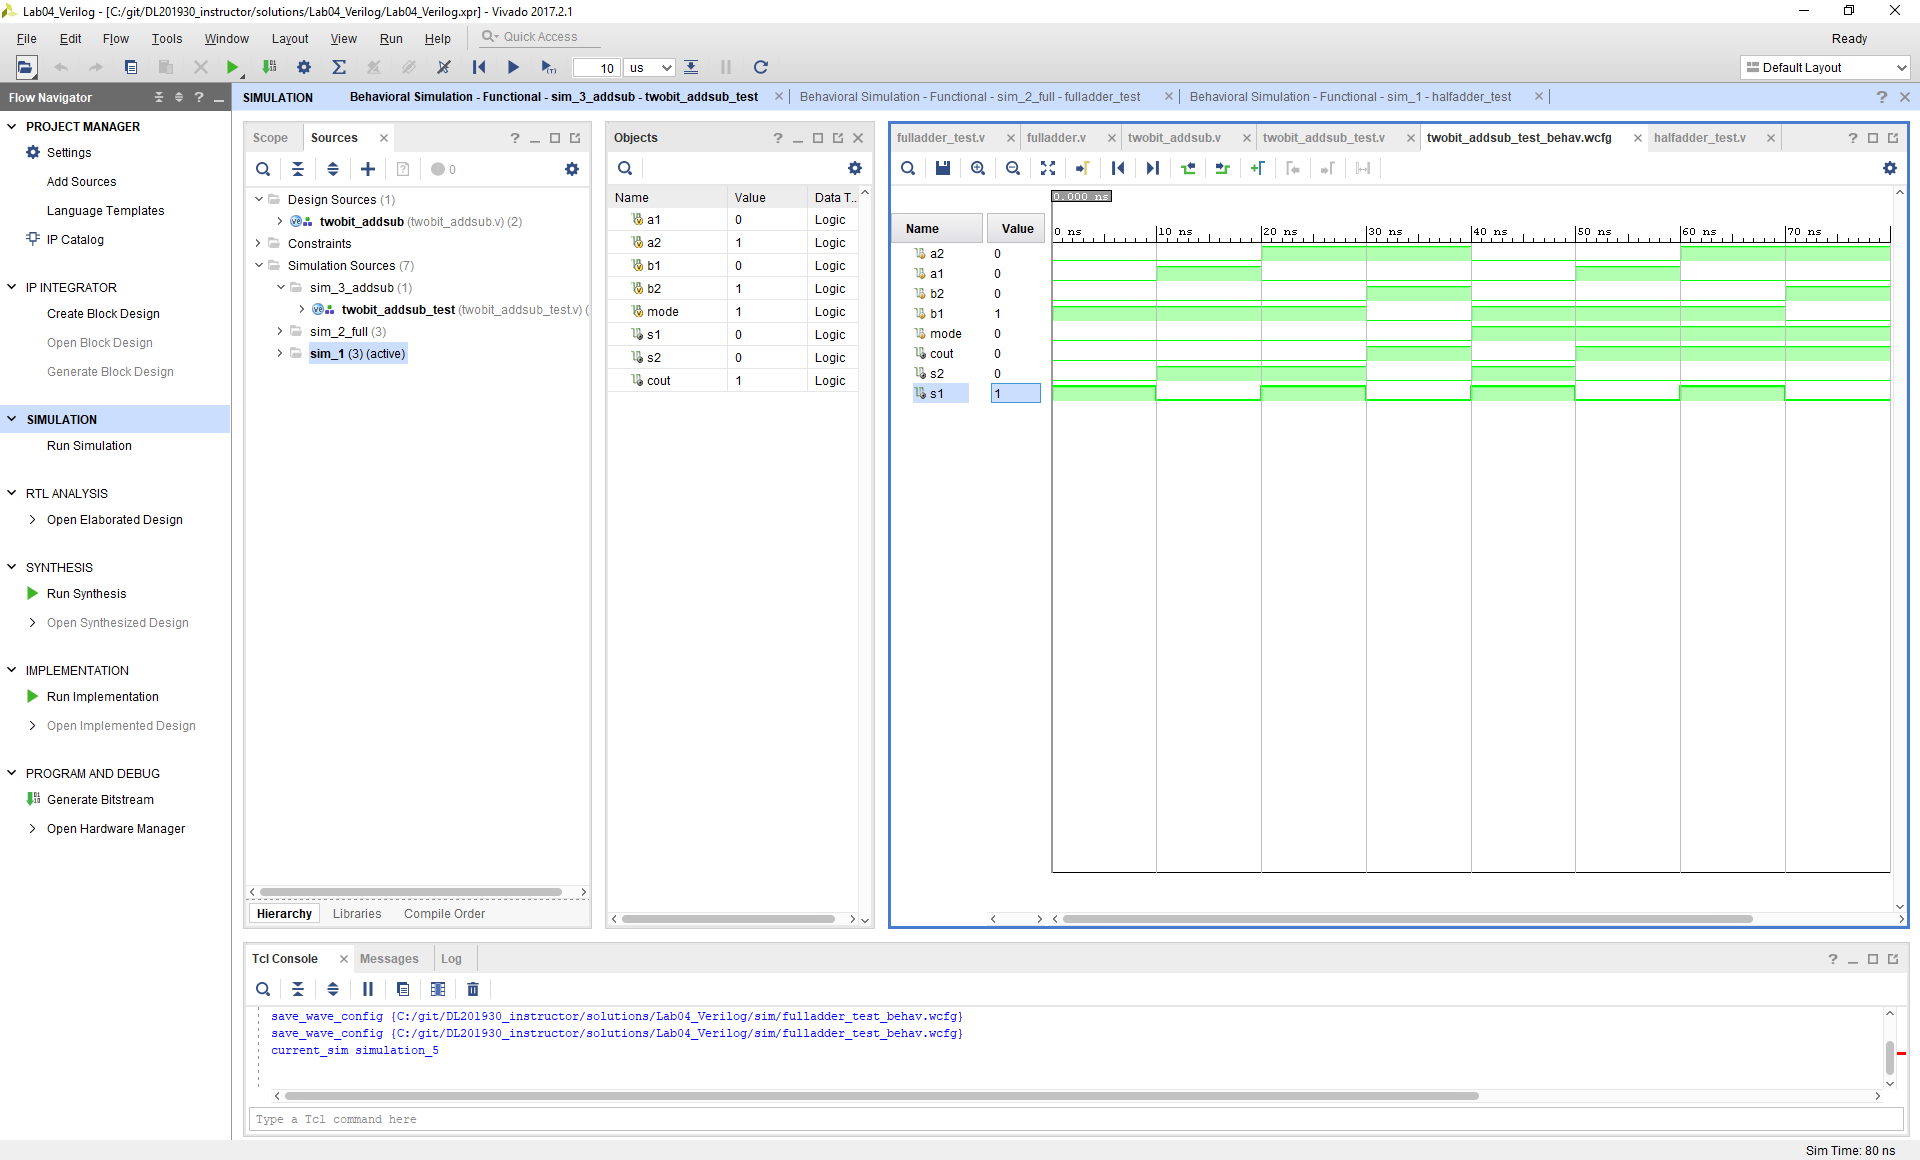
\includegraphics[width=1.0\textwidth]{Lab1Table}
		\caption{This is the original logo.}
		\label{fig:Lab1Table}
	\end{figure}
	
	\begin{figure}[ht]\centering
		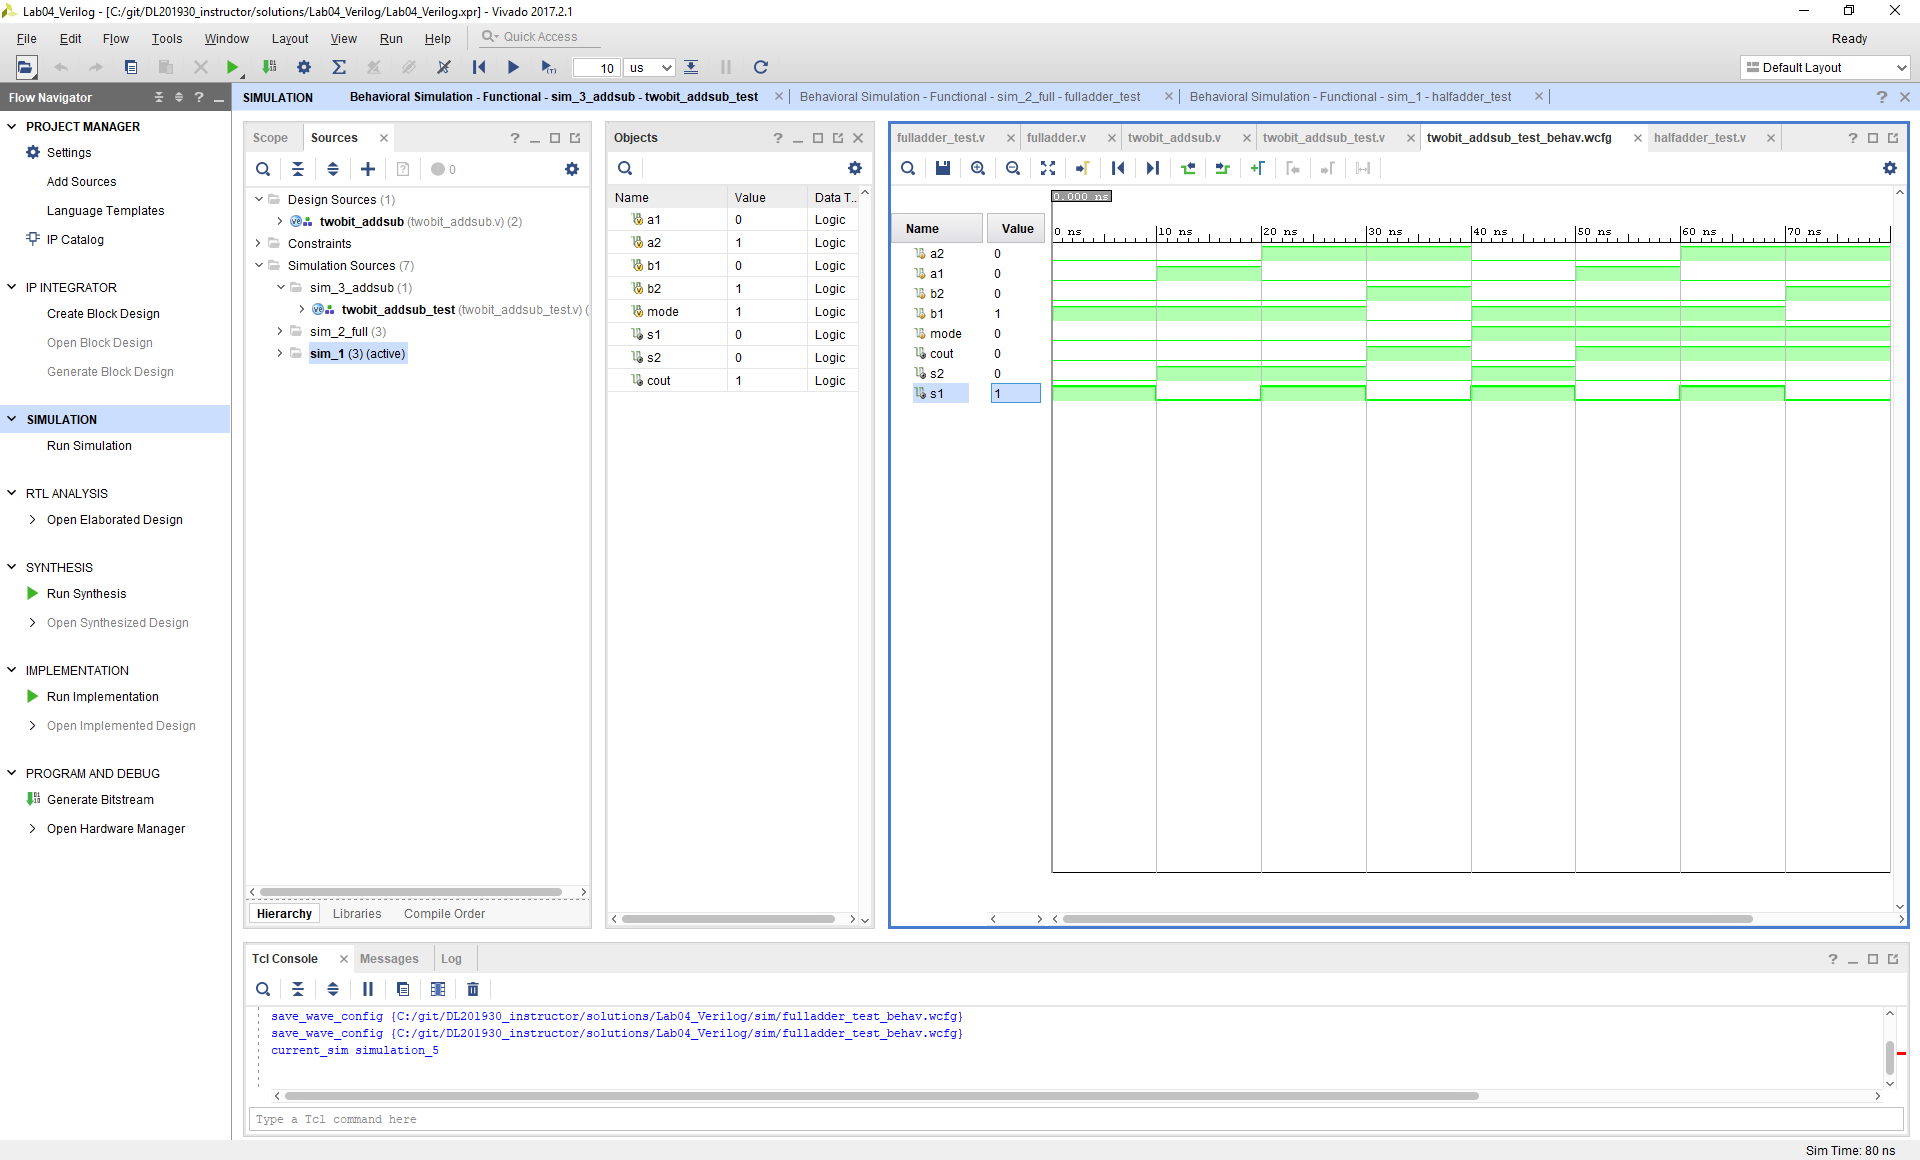
\includegraphics[width=1.0\textwidth,trim=8cm 8cm 0cm 0cm,clip]{Lab1Table}
		\caption{This is the logo cropping the top and bottom.}
		\label{fig:another_image}
	\end{figure}

	Figure 3 is the picture after I commit these changes to my repo and push them toGitHub. In GHD, the the History tab to show me all of my commits thus far.\\
	\begin{figure}[ht]\centering
		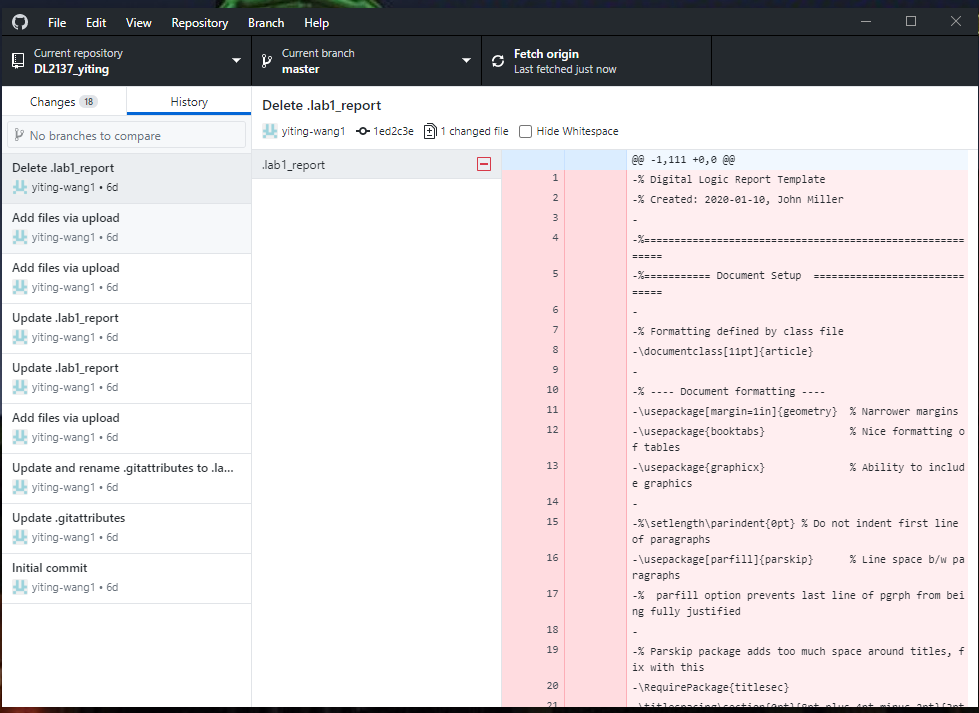
\includegraphics[width=1.0\textwidth]{GitHub}
		\caption{This is the screenshot of the GitHub History tab}
		\label{fig:GitHub}
	\end{figure}



\section*{Code}
	Here is the code including from examplecode.sv in the Code section.\\
	module example \\
	\#(parameter BITS=4) \\
	(\\
	input [BITS-1:0] in0, in1,\\
	input sel,\\
	output [BITS-1:0] out\\
	);\\
	
	// Choose in1 or in0\\
	out = sel ? in1: in0; \\
	endmodule



\end{document}
